%%% Hlavní soubor. Zde se definují základní parametry a odkazuje se na ostatní části. %%%

%% Verze pro jednostranný tisk:
% Okraje: levý 40mm, pravý 25mm, horní a dolní 25mm
% (ale pozor, LaTeX si sám přidává 1in)
\documentclass[12pt,a4paper]{report}
\setlength\textwidth{145mm}
\setlength\textheight{247mm}
\setlength\oddsidemargin{15mm}
\setlength\evensidemargin{15mm}
\setlength\topmargin{0mm}
\setlength\headsep{0mm}
\setlength\headheight{0mm}
% \openright zařídí, aby následující text začínal na pravé straně knihy
\let\openright=\clearpage

%% Pokud tiskneme oboustranně:
% \documentclass[12pt,a4paper,twoside,openright]{report}
% \setlength\textwidth{145mm}
% \setlength\textheight{247mm}
% \setlength\oddsidemargin{14.2mm}
% \setlength\evensidemargin{0mm}
% \setlength\topmargin{0mm}
% \setlength\headsep{0mm}
% \setlength\headheight{0mm}
% \let\openright=\cleardoublepage

%% Vytváříme PDF/A-2u
\usepackage[a-2u]{pdfx}

%% Přepneme na českou sazbu a fonty Latin Modern
\usepackage[czech]{babel}
\usepackage{lmodern}
\usepackage[T1]{fontenc}
\usepackage{textcomp}

%% Použité kódování znaků: obvykle latin2, cp1250 nebo utf8:
\usepackage[utf8]{inputenc}

%%% Další užitečné balíčky (jsou součástí běžných distribucí LaTeXu)
\usepackage{amsmath}        % rozšíření pro sazbu matematiky
\usepackage{amsfonts}       % matematické fonty
\usepackage{amsthm}         % sazba vět, definic apod.
\usepackage{amssymb}        % nejake symboly
\usepackage{bbding}         % balíček s nejrůznějšími symboly
			    % (čtverečky, hvězdičky, tužtičky, nůžtičky, ...)
\usepackage{bm}             % tučné symboly (příkaz \bm)
\usepackage{graphicx}       % vkládání obrázků
\usepackage{fancyvrb}       % vylepšené prostředí pro strojové písmo
\usepackage{indentfirst}    % zavede odsazení 1. odstavce kapitoly
\usepackage{natbib}         % zajištuje možnost odkazovat na literaturu
			    % stylem AUTOR (ROK), resp. AUTOR [ČÍSLO]
\usepackage[nottoc]{tocbibind} % zajistí přidání seznamu literatury,
                            % obrázků a tabulek do obsahu
\usepackage{icomma}         % inteligetní čárka v matematickém módu
\usepackage{dcolumn}        % lepší zarovnání sloupců v tabulkách
\usepackage{booktabs}       % lepší vodorovné linky v tabulkách
\usepackage{paralist}       % lepší enumerate a itemize
\usepackage[usenames]{xcolor}  % barevná sazba

\usepackage{placeins}

\usepackage{tikz}           % obrazky kvuli DNA
\usetikzlibrary{chains,fit,shapes,calc,arrows,backgrounds}

\usepackage{xstring}

%%% Údaje o práci

% Název práce v jazyce práce (přesně podle zadání)
\def\NazevPrace{Simulace dějů predikovaných teorií zamrzlé plasticity}

% Název práce v angličtině
\def\NazevPraceEN{Simulation of processes predicted by theory of frozen plasticity}

% Jméno autora
\def\AutorPrace{Bc. Ondřej Nekola}

% Rok odevzdání
\def\RokOdevzdani{2017}

% Název katedry nebo ústavu, kde byla práce oficiálně zadána
% (dle Organizační struktury MFF UK, případně plný název pracoviště mimo MFF)
\def\Katedra{Katedra filosofie a dějin přírodních věd}
\def\KatedraEN{Department of Philosophy and History of Science}

% Jedná se o katedru (department) nebo o ústav (institute)?
\def\TypPracoviste{Katedra}
\def\TypPracovisteEN{Department}

% Vedoucí práce: Jméno a příjmení s~tituly
\def\Vedouci{prof. RNDr. Jaroslav Flegr, CSc.}

% Pracoviště vedoucího (opět dle Organizační struktury MFF)
\def\KatedraVedouciho{katedra}
\def\KatedraVedoucihoEN{department}

% Studijní program a obor
\def\StudijniProgram{Biologie}
\def\StudijniObor{Teoretická a evoluční biologie}

% Nepovinné poděkování (vedoucímu práce, konzultantovi, tomu, kdo
% zapůjčil software, literaturu apod.)
\def\Podekovani{%
Poděkování. XXXX
}

% Abstrakt (doporučený rozsah cca 80-200 slov; nejedná se o zadání práce)
\def\Abstrakt{%
Abstrakt. XXXX
}
\def\AbstraktEN{%
Abstract. XXXX
}

% 3 až 5 klíčových slov (doporučeno), každé uzavřeno ve složených závorkách
\def\KlicovaSlova{%
{klíčová} {slova} XXXX
}
\def\KlicovaSlovaEN{%
{key} {words} XXXX
}

%% Balíček hyperref, kterým jdou vyrábět klikací odkazy v PDF,
%% ale hlavně ho používáme k uložení metadat do PDF (včetně obsahu).
%% Většinu nastavítek přednastaví balíček pdfx.
\hypersetup{unicode}
\hypersetup{breaklinks=true}

%% Definice různých užitečných maker (viz popis uvnitř souboru)
%%% Tento soubor obsahuje definice různých užitečných maker a prostředí %%%
%%% Další makra připisujte sem, ať nepřekáží v ostatních souborech.     %%%

%%% Drobné úpravy stylu

% Tato makra přesvědčují mírně ošklivým trikem LaTeX, aby hlavičky kapitol
% sázel příčetněji a nevynechával nad nimi spoustu místa. Směle ignorujte.
\makeatletter
\def\@makechapterhead#1{
  {\parindent \z@ \raggedright \normalfont
   \Huge\bfseries \thechapter. #1
   \par\nobreak
   \vskip 20\p@
}}
\def\@makeschapterhead#1{
  {\parindent \z@ \raggedright \normalfont
   \Huge\bfseries #1
   \par\nobreak
   \vskip 20\p@
}}
\makeatother

% Toto makro definuje kapitolu, která není očíslovaná, ale je uvedena v obsahu.
\def\chapwithtoc#1{
\chapter*{#1}
\addcontentsline{toc}{chapter}{#1}
}

% Trochu volnější nastavení dělení slov, než je default.
\lefthyphenmin=2
\righthyphenmin=2

% Zapne černé "slimáky" na koncích řádků, které přetekly, abychom si
% jich lépe všimli.
\overfullrule=1mm

%%% Makra pro definice, věty, tvrzení, příklady, ... (vyžaduje baliček amsthm)

\theoremstyle{plain}
\newtheorem{veta}{Věta}
\newtheorem{lemma}[veta]{Lemma}
\newtheorem{tvrz}[veta]{Tvrzení}

\theoremstyle{plain}
\newtheorem{definice}{Definice}

\theoremstyle{remark}
\newtheorem*{dusl}{Důsledek}
\newtheorem*{pozn}{Poznámka}
\newtheorem*{prikl}{Příklad}

%%% Prostředí pro důkazy

\newenvironment{dukaz}{
  \par\medskip\noindent
  \textit{Důkaz}.
}{
\newline
\rightline{$\square$}  % nebo \SquareCastShadowBottomRight z balíčku bbding
}

%%% Prostředí pro sazbu kódu, případně vstupu/výstupu počítačových
%%% programů. (Vyžaduje balíček fancyvrb -- fancy verbatim.)

\DefineVerbatimEnvironment{code}{Verbatim}{fontsize=\small, frame=single}

%%% Prostor reálných, resp. přirozených čísel
\newcommand{\R}{\mathbb{R}}
\newcommand{\N}{\mathbb{N}}

%%% Užitečné operátory pro statistiku a pravděpodobnost
\DeclareMathOperator{\pr}{\textsf{P}}
\DeclareMathOperator{\E}{\textsf{E}\,}
\DeclareMathOperator{\var}{\textrm{var}}
\DeclareMathOperator{\sd}{\textrm{sd}}

%%% Příkaz pro transpozici vektoru/matice
\newcommand{\T}[1]{#1^\top}

%%% Vychytávky pro matematiku
\newcommand{\goto}{\rightarrow}
\newcommand{\gotop}{\stackrel{P}{\longrightarrow}}
\newcommand{\maon}[1]{o(n^{#1})}
\newcommand{\abs}[1]{\left|{#1}\right|}
\newcommand{\dint}{\int_0^\tau\!\!\int_0^\tau}
\newcommand{\isqr}[1]{\frac{1}{\sqrt{#1}}}

%%% Vychytávky pro tabulky
\newcommand{\pulrad}[1]{\raisebox{1.5ex}[0pt]{#1}}
\newcommand{\mc}[1]{\multicolumn{1}{c}{#1}}


\pgfdeclarelayer{background layer}
\pgfdeclarelayer{foreground layer}
\pgfsetlayers{background layer,main,foreground layer}


\newcommand*{\NodeSize}{0.8cm}%
\newcommand*{\YShiftBetweenRows}{-1cm}% Subsequent rows are shited down so they don't overlap
\tikzset{DNA Style/.style={minimum size=0.8cm, draw=gray, line width=1pt}}

\tikzset{Fit Line Style 1/.style={draw=olive, thick, dotted}}
\tikzset{Fill Style 1/.style={fill=olive!20}}

\tikzset{Fit Line Style 2/.style={draw=green!50!black, thick, dashed}}
\tikzset{Fill Style 2/.style={fill=green!20}}

\newlength{\YShift}% 
\newcounter{ColumnCounter}% Prefix for node labels

% Initialize - These are probably not needed, but prefer to set them
\setlength{\YShift}{0cm}% 
\setcounter{ColumnCounter}{0}


\newcommand*{\DNASequence}[2][Mark]{%
    % http://tex.stackexchange.com/questions/12091/tikz-foreach-loop-with-macro-defined-list
    \setcounter{ColumnCounter}{0}
    \def\Sequence{#2}
    \foreach [count=\xi] \Label/\Color in \Sequence {%
        \pgfmathsetmacro{\XShift}{\NodeSize*\xi}%
        \IfStrEq{\Color}{}{\def\Color{white}}{}
        \edef\NodeName{#1-\arabic{ColumnCounter}}
        \begin{pgfonlayer}{foreground layer}
        \node [DNA Style, fill=\Color, xshift=\XShift] (\NodeName) {\Label};
        \end{pgfonlayer}
        \stepcounter{ColumnCounter}
    } 
}%


\newcommand*{\ConnectNodes}[3][]{%
    % #1 = draw options
    % #2 = ending node
    % #3 = list of starting nodes
    \def\ListOfEndNodes{#3}
    \foreach \EndNode in \ListOfEndNodes {%
    \draw[latex'-, thin, #1] (#2) to[#1] (\EndNode);
    }%
  }

\begin{document}
%%% Titulní strana práce a další povinné informační strany

%%% Titulní strana práce

\pagestyle{empty}
\hypersetup{pageanchor=false}

\begin{center}

{\bf\Large Univerzita Karlova}

\vspace{4mm}

{\bf\Large Přírodovědecká fakulta}


\vspace{10mm}

\begin{tabular}{rl}
\Large Studijní program: & \Large\StudijniProgram \\
\noalign{\vspace{2mm}}
\Large Studijní obor: & \Large\StudijniObor \\
\end{tabular}


\vfill

\begin{figure}[h]
\centering
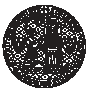
\includegraphics[width=16em]{img/znak.pdf}
\end{figure}

\vfill

{\Large\bf\AutorPrace}

\vspace{15mm}

{\Large\NazevPrace}

\vspace{4mm}

{\Large\NazevPraceEN}

\vfill


\begin{tabular}{rl}
\Large Typ závěrečné práce: & \Large Diplomová práce \\
\noalign{\vspace{4mm}}
\Large Vedoucí práce: & \Large\Vedouci \\
\end{tabular}

\vfill

% Zde doplňte rok
{\Large Praha \RokOdevzdani }

\end{center}

\newpage

%%% Následuje vevázaný list -- kopie podepsaného "Zadání diplomové práce".
%%% Toto zadání NENÍ součástí elektronické verze práce, nescanovat.

%%% Strana s čestným prohlášením k diplomové práci

\openright
\hypersetup{pageanchor=true}
\pagestyle{plain}
\pagenumbering{roman}
\vglue 0pt plus 1fill

\noindent
Prohlašuji, že jsem tuto diplomovou práci vypracoval samostatně a výhradně
s~použitím citovaných pramenů, literatury a dalších odborných zdrojů.

\medskip\noindent
Beru na~vědomí, že se na moji práci vztahují práva a povinnosti vyplývající
ze zákona č. 121/2000 Sb., autorského zákona v~platném znění, zejména skutečnost,
že Univerzita Karlova má právo na~uzavření licenční smlouvy o~užití této
práce jako školního díla podle §60 odst. 1 autorského zákona.

\vspace{10mm}

\hbox{\hbox to 0.5\hsize{%
V Praze dne 29.8.2017
\hss}\hbox to 0.5\hsize{%
Ondřej Nekola
\hss}}

\vspace{20mm}
\newpage

%%% Poděkování

\openright

\noindent
\Podekovani

\newpage

%%% Povinná informační strana diplomové práce

\openright

\vbox to 0.5\vsize{
\setlength\parindent{0mm}
\setlength\parskip{5mm}

Název práce:
\NazevPrace

Autor:
\AutorPrace

\TypPracoviste:
\Katedra

Vedoucí diplomové práce:
\Vedouci, \KatedraVedouciho

\vss}\nobreak\vbox to 0.49\vsize{
\setlength\parindent{0mm}
\setlength\parskip{5mm}

Title:
\NazevPraceEN

Author:
\AutorPrace

\TypPracovisteEN:
\KatedraEN

Supervisor:
\Vedouci, \KatedraVedoucihoEN

\vss}

\newpage

Abstrakt:
\Abstrakt

\vspace*{3em}

Klíčová slova:
\KlicovaSlova

\newpage

Abstract:
\AbstraktEN

\vspace*{3em}

Keywords:
\KlicovaSlovaEN

\newpage

\openright
\pagestyle{plain}
\pagenumbering{arabic}
\setcounter{page}{1}


%%% Strana s automaticky generovaným obsahem diplomové práce

\tableofcontents

%%% Jednotlivé kapitoly práce jsou pro přehlednost uloženy v samostatných souborech
\include{0_uvod}
\chapter{Literární přehled}

\section{Název první podkapitoly v druhé kapitole}

\section{Název druhé podkapitoly v druhé kapitole}


\chapter{Metodika}


%V této části buďte velmi precizní. Vše musíte popsat tak důkladně, aby kdokoliv mohl vaše pokusy či
%pozorování zopakovat. Nezapomeňte uvést velikost vzorků, věk a pohlaví zvířat, denní a roční dobu,
%podmínky chovu nebo popis lokalit (třeba včetně mapky), specifické přístrojové vybavení
%(pokud je to důležité, např.~pro srovnání výsledků s publikovanými údaji, uveďte i přesný typ
%přístroje) a jiné podrobnosti. Také může být dobré zmínit, jak jste zabránili vlivu pakovaného testování stejných
%individuí a proč se domníváte, že je počet jedinců dostatečný k zodpovězení vašich otázek. Více než
%vhodné je zmínit a zdůvodnit použité statistické metody a počítačové programy. Používáte-li zkratky, uveďte
%jejich seznam.
%Materiál a metodika bývají pro větší srozumitelnost často členěny na menší podkapitoly: materiál,
%experimentální design, analýza dat atd. Systém více podkapitol třeba jen o třech řádcích bývá přehlednější
%než souvislý odstavec na dvě strany. (A to samozřejmě neplatí jen pro metodiku.)
%Čtení DP usnadní, pokud je členění na podkapitoly obdobné v kapitolách Materiál a metodika,
%Výsledky a případně i Diskuse.
%Při vší pečlivosti se však snažte být poměrně struční. Materiál a metodika by neměly tvořit většinu DP.

XXX neco trosku obecnejsiho?

\section{Simulace}

Použil jsem stochastický model postavený na individuích. Individua jsou jedinci jednoho druhu s oddělenými pohlavími a
žijí v nestrukturovaném prostředí. Fenotyp jedinců i optimum prostředí jsou čtyřrozměrnými vektory.
Optimum prostředí $E(t)$ není stálé, ale může se měnit v čase.
Euklidovská vzdálenost fenotypu jedince od aktuálního optima prostředí určuje jeho fitness.

Optimum prostředí je po dobu 2048 kroků simulace konstantní a následně dojde k jeho skokové změně o
$\Delta{}E$. Po této změně opět zůstane optimum neměnné.

Počáteční velikost populace je jedním z parametrů simulace. V~dalších krocích je následně velikost populace udržována
mechanismem turbidostatu.
Navíc je každý jedinec limitován maximální délkou života -- po 64 (XXX) krocích umírá.
Jedinci jsou sexuálně dospělí ihned v následujícím kroku simulace a věk neovliňuje jejich fenotyp.



XXX picture: Big picture



V každém kroku jsou z populace náhodně vybrány páry opačného pohlaví a osmina z nich se může rozmnožit.
Kolik vyvedou potomků, je určeno průměrnou fitness páru. Způsob, jak je jsou určeny počty potomků, jejich geny a
jak následně geny určují jejich fenotyp, je popsán později.
Při každém kroku simulace také velmi malou část jedinců postihne mutace jednoho nebo více genů.

\section{Jedinec a jeho geny}

Geny každého jedince jsou uloženy v dvou homologních chromosomech. Každý z těchto chromosomů má XXX lokusů.
Na každém z lokusů je alela, která má vliv na fenotyp jedince. Alela je určena svým příspěvkem k fenotypu (čtyřrozměrný
vektor, typicky s jednou nenulovou hodnotou) a svým příspěvkem k fenotypu, pokud se vyskytuje na obou protilehlých
lokusech (opět čtyřrozměrný vektor). Druhý příspěvek k fenotypu se tedy projevuje jako dominance alely.

Na počátku simulace jsou vygenerováni náhodní jedinci. Jejich alely jsou generovány náhodně - příspěvek k fenotypu
má jednu nenulovou složku pro náhoně zvolenou dimenzi. Velikost této složky je vybrána z normálního rozdělení. Vliv na
fenotyp v případě dominance závisí na parametrech simulace. S určenou pravěpodobností je to opačný vektor k běžnému
vlivu na fenotyp, jinak je to nulový vektor.

\subsection{Mutace}

Jedinou možnou mutací je změna alely za jinou - nejsou tedy simulovany rozsahlejsi mutace, ktere maji vetsi vliv na
strukturu DNA.

Nad každým lokusem v obou chromosomech určeno s pravděpodobností XXX, zda u něj dojde ke změně.
V případě, že ano, tak je na lokus dána nová náhodná. Nová alela vybírána obdobným mechanismem, jako jsou
generovny počáteční alely.

\begin{figure}
  \centering

  \begin{tikzpicture}

    \begin{scope}
      \DNASequence[Mutated]{$\blacktriangleright$/white!30,$\clubsuit$/red!30,$\#$/white!30,$\triangleleft$/white!30,$\circ$/white!30,$\flat$/white!30}
    \end{scope}

    \begin{scope}[yshift=1cm]
      \DNASequence{$\triangleright$/white!20,$\clubsuit$/white!30,$\bot$/white!20,$\triangleleft$/white!30,$\bullet$/white!30,$\sharp$/white!30}
    \end{scope}


    \begin{scope}[xshift=9cm]
      \DNASequence[Done]{$\blacktriangleright$/white!30,$\diamondsuit$/red!30,$\#$/white!30,$\triangleleft$/white!30,$\circ$/white!30,$\flat$/white!30}
    \end{scope}

    \begin{scope}[xshift=9cm,yshift=1cm]
      \DNASequence{$\triangleright$/white!20,$\clubsuit$/white!30,$\bot$/white!20,$\triangleleft$/white!30,$\bullet$/white!30,$\sharp$/white!30}
    \end{scope}

    \ConnectNodes[out=-90, in=-30]
        {Done-1.south}
        {Mutated-1.south};

  \end{tikzpicture}

  \caption{Mutace}
\end{figure}

\subsection{Křížení}

Každý jedinec má jedno ze dvou pohlaví. V každém kroku simulace jsou náhodně vytvořeny páry jedinců opačného pohlaví.

Náhodě vybraná osmina párů má následně možnost splodit potomky.

Každý z potomků vzniká tak, že jsou kombinovány geny obou rodičů. Pro každý chromozom je vybrán náhodný lokus.
Lokusy před ním a on jsou naplněny alelami jednoho z rodičů, lokusy po něm alelami druhého z rodičů.

Pohlaví potomka je určeno náhodně se stejnou pravděpodobností pro obě pohlaví.

\begin{figure}
  \centering

  \begin{tikzpicture}

    \begin{scope}
      \DNASequence[Parent1a]{$\blacktriangleright$/yellow!30,$\clubsuit$/yellow!30,$\boxplus$/yellow!30,$\circ$/yellow!30,$\circledcirc$/yellow!30,$\flat$/yellow!30}
    \end{scope}

    \begin{scope}[yshift=1cm]
      \DNASequence[Parent1b]{$\triangleright$/yellow!20,$\diamondsuit$/yellow!30,$\boxdot$/yellow!20,$\bullet$/yellow!30,$\circledcirc$/yellow!30,$\flat$/yellow!30}
    \end{scope}


    \begin{scope}[yshift=3cm]
      \DNASequence[Parent2a]{$\blacktriangle$/green!30,$\clubsuit$/green!30,$\boxdot$/green!30,$\star$/green!30,$\circledcirc$/green!30,$\flat$/green!30}
    \end{scope}

    \begin{scope}[yshift=4cm]
      \DNASequence[Parent2b]{$\triangle$/green!20,$\clubsuit$/green!30,$\Box$/green!20,$\ast$/green!30,$\circledcirc$/green!30,$\sharp$/green!30}
    \end{scope}

    \begin{scope}[xshift=9cm,yshift=2cm]
      \DNASequence[Donea]{$\blacktriangle$/green!30,$\clubsuit$/green!30,$\boxplus$/yellow!30,$\circ$/yellow!30,$\circledcirc$/yellow!30,$\flat$/yellow!30}
    \end{scope}

    \begin{scope}[xshift=9cm,yshift=3cm]
      \DNASequence[Doneb]{$\triangle$/green!20,$\clubsuit$/green!30,$\Box$/green!20,$\ast$/green!30,$\circledcirc$/green!30,$\flat$/yellow!30}
    \end{scope}

    \ConnectNodes[out=-90, in=-30]
        {Donea-3.south}
        {Parent1a-3.south};

    \ConnectNodes[out=-90, in=-0]
        {Donea-0.south east}
        {Parent2a-0.south east};

    \ConnectNodes[out=90, in=40]
        {Doneb-2.north}
        {Parent2b-2.north};

    \ConnectNodes[out=90, in=40]
        {Doneb-5.north}
        {Parent1b-5.north};

  \end{tikzpicture}

  \caption{Křížení}
\end{figure}



\section{Jedinec a jeho fenotyp}

Fenotyp jedince jsou jeho čtyři kvantitativní vlastnosti dohromady reprezentované jako čtyřrozměrný vektor.

Každá alela nějak přispívá do výsledného fenotypu, tyto příspěvky se sčítají. Příspěvek alely se může lišit, pokud se
nachází ve dvou kopiích na protilehlých lokusech.

Aby simulace postihla různé procesy, které komplikují to, jak genotyp určuje fenotyp, je na jejím začátku
vygenerováno množství pravidel, která v závislosti na přítomnosti různých kombinací alel mění výsledný fenotyp.
Jmenovitě jde o epistatické interakce, pleiotropii a dominanci.

Každé pravidlo se skládá z předpokladů a vlivu na fenotyp. Příkladem složitějšího pravidla, v tomto případě
epistatického \uv{pokud alespoň jeden z chromosomů obsahuje na lokusu $3$ alelu s danými vlastnostmi (XXX) a alespoň
jeden z chromosomů obsahuje na lokusu $7$ alelu s jinými vlastnostmi (XXX), tak změň výsledný fenotyp o $[0, 0, 0, -0.431]$} .

Fenotyp jedince je tak určen jako (vektorový) součet příspěvků pravidel,
jejichž předpokladům geny jedince vyhovují a součtu příspěvků jednotlivých alel.
Každá složka fenotypu tak může být ovlivněna více geny a naopak každý gen může mít, často jen ve souhře s jinými geny,
vliv na různé složky fenotypu.

Obr XXX znázornění předpokladů pravidla

Obr XXX znázornění situace, kdy jedinec odpovídá pravidlu

Obr XXX znázornění situace, kdy jedinec neodpovídá pravidlu

Počty jednotlivých pravidel patří mezi parametry simulace.

\footnote{Seznam všech parametrů simulace je součástí přílohy XXX}

\subsection{Jednoduché příspěvky od alel}

Jednoduché pravidlo zachycuje příspěvek jedné alely k jedné složce fenotypu.

Obr XXX

Na počátku je pro každý lokus vybrána náhodná dimenze, kterou budou alely v ní ovlivňovat. Pro každou alelu pak změna
fenotypu má jednu nenulovou hodnotu v náhodně vybrané dimenzi. Velikost této změny je vybrána z normálního rozložení,
vlivy jednotlivých alel ze stejného locusu se tak mohou lišit jak ve směru, tak ve velikosti.

\subsection{Pravidla pro pleiotropii a epistázi}

Společný vliv kombinace více alel -- typicky na různých lokusech -- na fenotyp odlišný od pouhého součtu příspěvků samostatných alel bývá nazýván epistatickou interakcí.

Epistatická pravidla mají, stejně jako jednoduchá pravidla, ve svém vektoru vlivu na fenotyp jen jednu nenulovou hodnotu. Pro každé pravidlo je vybrána náhodná dimenze a velikost vlivu je vybrána z normálního rozložení.

Naopak pleiotropní pravidla popisují situaci, kdy jedna alela ovlivňuje více vlastností. Každé takové pravidlo má podmínku obsahující jedinou alelu a vliv na fenotyp obsahující čtyři čísla, každé vybrané z normálního roložení.

Počet epistatických a počet pleiotropických pravidel jsou parametry simulace.

\subsection{Pravidla pro dominanci}

Pravidla postihující vztah dominance mezi alelami mají podobnou strukturu jako ostatní pravidla. Liší se jejich podmínka -- tou je společný výskyt dvou konkrétních alel na XXX lokusech na obou chromosomech. Pokud je podmínkou výskyt $G_i{2}$ a $G_i{3}$, tak je lhostejné, zda se obeví G2 na \textit{i}-tém lokusu prvního chromosomu a G3 na \textit{i}-tém lokusu druhého chromosomu nebo naopak.

XXX obrazek

Existují dvě zajímavé skupiny dominantních vztahů. Jednou je situace, kdy vliv dvou výskytů téže alely je u homozygototů výrazně větší než u vliv téže osamělé alely u heterozygotů. Druhou je, pokud vliv dvou výskytů téže alely působí u homozygotů v opačném směru, než její osamocený výskyt u heterozygotů.



\section{Optimum}

Pro simulovaný druh existuje optimální fenotyp, který nejlépe vyhovuje aktuálnímu stavu prostředí. Tento optimální fenotyp se v průběhu simulace jednou skokově -- v jejím kroku číslo 2048 -- změní.

Počáteční optimum je nastaveno na osminásobek výběru z normálního roložení nezávisle pro každou dimenzi. Změna proběhne o šestnáctinásobek výběru z normálního rozložení nezávisle pro každou dimenzi.

XXX
$$
E(0) =  [8{\cdot}X_1, 8{\cdot}X_2, 8{\cdot}X_3, 8{\cdot}X_4], F(X_i) \sim \phi
$$

$$
\Delta{E} = [8{\cdot}X_1, 8{\cdot}X_2, 8{\cdot}X_3, 8{\cdot}X_4], F(X_i) \sim \phi
$$

$$
E(t) = \left \{
     \begin{array}{l} E(0), \quad t \leq 2048 \\
                      E(0) + \Delta{E}, \quad jinak
\end{array} \right .
$$

\subsection{Fitness}

Euklidovská vzdálenost jedince s fenotypem $X = [X_1,\dots{}X_4]$ od aktuálního optima prostředí určuje
$E = [E_1,\dots{} E_4]$ jeho aktuální fitness, tak jak bylo zavedeno ve Fisherově geometrickém modelu XXX
\footnote{Konstanta $a$ v tomto vzorci jsou čistě empiricky zvolená tak, aby, měli jedinci v simulacích
přiměřené velikosti fitness -- pokud by například místo ní byla výrazně větší konstanta, tak by pro většinu simulací
neměla většina párů potomky a druh by v nich brzy vymřel. Což je nezajímavé a neodpovídá to reálným druhům.
Dvojka v exponentu je pak ve fisherovkých modelech běžná volba[XXX].
Seznam všech konstant, jak byly voleny pro simulace, je součástí přílohy XXX.}

$$fitness = 4{\cdot}e^{-a |E-X|^2} = 4{\cdot}e^{-a\cdot{\sum{(E_i - X_i)^2}}}$$

Počet potomků páru je aritmetický průměr fitness jeho členů zaokrouhlený dolů.


\section{Řízení velikosti populace}

Počáteční velikost populace je jedním z parametrů simulace. Následně je velikost populace řízena turbidostatickou
zpětnou vazbou[XXX]. V každém kroku má v populaci s $n$ jedinci každý jedinec pravděpodobnost
$p = min(0.9, k_4 n^2 + k5)$, že zahyne. Člen $k_4 n^2$ závisí na čtverci velikosti populace, a tedy její hustotě.
V přírodě mu odpovídá například regulace parazitem, kterému se lépe daří, pokud se jedinci častěji setkávají.
Člen $k5$ je pravděpodobnost náhodného úmrtí nezávislého na velikosti populace. Pravděpodobnost je z praktických důvodů
zastropována hodnotou 0.9 -- bez tohoto omezení by mohla s $n$ růst nade všechny meze a tedy i nad $1$, kde se ztrácí
možnost (nejen biologické) interpretace.
\footnote{Vzorec pro turbidostatickou regulaci očividně odpovídá realitě jenom pro aktuální velikosti populace,
které řádově nepřekračují rovnovážnou velikost populace. Omezení pravděpodobnosti pod $0.9$ v představovaných
simulacích postačuje pro postupný pokles k očekávané velikosti populace, protože počet potomků je omezený a
menší než deset na pár. XXX}

Konstanta $k4$ v předchozím vzorci je vypočítána následově: $XXX$. Pro simulace byla zvolena nulová pravděpodobnost
náhodného úmrtí $k5$ a řízení velikosti populace tedy záviselo jen na její hustotě a na deterministické smrti
stářím po $64$ XXX generacích.


\section{Frozen Beagle}

Popsaná simulace byla implementována v silně staticky typovaném čistě funkcionálním jazyce Haskell \cite{Haskell}.

Samotná simulace je zapouzdřena do knihovny, která je užívána dvěma programy -- grafickým
\textit{FrozenBeagleSimulation} a \textit{fbeagle}, který je spouštěn z příkazové řádky.

Grafický \textit{FrozenBeagleSimulation}, zobrazený na XXX,
umožňuje pohodlně nastavit parametry simulace a jednu spustit.



\begin{figure}
\centering
\includegraphics[totalheight=8cm]{img/ukazka-obr01.pdf}
    \caption{FrozenBeagleSimulation screenshot}
\end{figure}


\textit{fbeagle} je vhodný pro dávkové zpracování, které spouští mnoho simulací se stejnými parametry, které se liší počátečním \textit{seedem} generátoru pseudonáhodných čísel. Jeho výstupem je sada statistik pro jednotlivé simulace, které je moźné dále analyzovat a zpracovávat.

Na adrese \url {https://github.com/satai/FrozenBeagle} jsou volně k dispozici zdrojové texty včetně jednotkových testů a kompletní historie ve VCS git. Jsou poskytnuty pod trojsložkovou BSD licencí.

\section{Statistická analýza}

\section{Reprodukovatelnost}

Bla, bla.

K sazbě byl použit systém \TeX se sadou maker \LaTeX a za použití fontů Latin Modern.

\chapter{Výsledky}

V DP uveďte všechny zjištěné výsledky včetně výsledků pilotních experimentů. Důkladně však zvažte, jaká část vašich výsledků má být prezentována v kapitole Výsledky. Měly by tu být především výsledky, které čímsi přispívají k zodpovězení vašich otázek. Základní data (např. tabulky naměřených rozměrů nebo genotypy jedinců)  patří spíše do Příloh nebo na přiložené CD. 

Mějte na paměti, že obrázky spíše vyjadřují myšlenky, zatímco tabulky zobrazují data. Údaje z tabulek neuvádějte znovu v textu. Pozor také na duplikaci údajů obsažených v tabulkách a grafech. Každá tabulka a graf však musí být v textu zmíněny (zjednodušeně řečeno: tabulka ukáže data, která jsou dále okomentována v textu).

Příklad: V tabulce číslo 1 jsou naměřené délky žížal v cm (10  10,1  10,7  10,9  11).  V textu se pak například objeví: ...z Tabulky 1 vyplývá, že žížaly měřily od 10 do 11cm...

Tabulky i obrázky by měly být očíslovány a podle čísel taky seřazeny (tedy Tabulka 1 se v textu objeví dříve než Tabulka 2).

Věnujte také zvýšenou pozornost popiskům obrázků a tabulek, které musí být \uv{self-explanatoryi}  a zkontrolujte popis os v grafech. Tabulky by měly být co nejjednodušší. Vertikální čáry vnich nejlépe nepoužívejte vůbec a počet čar horizontálních omezte na minimum.

Musí být zřejmé, nejen které statistické testy byly použity, ale také zda jsou pro ně splněny předpoklady (např. normální rozložení, pokud to test vyžaduje). 

Samozřejmě můžete použít barevné grafy či tabulky. Je ale dobré si uvědomit, že se hodnotí obsah, nikoliv barevnost. Klidně tedy vystačíte i jen s černou a bílou barvou (to samozřejmě nemusí platit pro fotografie nebo obrázky). Pokud použijete barevné grafy, měly by být (pokud možno) rozlišitelné i v černobílém provedení.

\section{Název první podkapitoly v druhé kapitole}

\section{Název druhé podkapitoly v druhé kapitole}


\chapter{Diskuse}

%
%Diskusi nepodceňujte. Je to nejdůležitější část a podle toho taky nejsložitější na napsání. Může se stát, že po napsání Diskuse budete muset přepsat třeba celý Úvod. Napsání kvalitní Diskuse vyžaduje spoustu času. Počítejte s tím. Za jeden večer to nenapíšete.
%
%Citát: \uv{Z krátké diskuse čiší stupidita autora, který vlastně neví co diskutovat.} Dr. B. Mandák, botanický ústav AVČR
%
%Bývá dobré začít shrnutím a interpretací vašich výsledků. Diskuse ale musí také ukázat jak výsledky zapadají do toho, co je o dané problematice známo. Musíte oddiskutovat jak soulad získaných výsledků s publikovanými tak i jejich nesoulad. Domníváte-li se, že jsou vaše výsledky zcela nové, pak vysvětlete v čem je jejich originalita. Pokud je nesoulad mezi výsledky vašimi a jiných badatelů, pak je nutné vysvětlit, čím k tomu mohlo dojít.
%
%Příklad: Sonntag (2001) sice uvádí, že by žížala mohla být i celkem krátká, neměl však k dispozici přesné měřítko, kterým žížalu měřím já.
%
%Nezapomeňte, že jste si v Úvodu vytyčili otázky a cíle. Na ně je třeba reagovat. Můžete i naznačit, jakým směrem by se teď po vašich zásadních objevech měl ubírat další výzkum. Můžete i formulovat nové hypotézy, které by měly být v budoucnu testovány. Pořadí diskutovaných okruhů by mělo být stejné jako bylo v Úvodu. Čtenář DP by měl být na Diskusi připraven Úvodem. Nemělo by se tedy stát, že se v Diskusi zjeví překvapivá fakta z prací jiných autorů, o nichž není v Úvodu ani zmínky.

XXXXX


\section{Název první podkapitoly v druhé kapitole}

XXX

\section{Název druhé podkapitoly v druhé kapitole}


\chapter*{Závěr}

% Stručně uveďte, co nového vaše DP přináší.
%Zmiňte jen ty nejdůležitější výsledky. Jedná se o souhrn výsledků.
%Neopakujte tedy fakta z Materiálu a metodiky.
%Po přečtení souhrnu by mělo být každému zcela jasné, o čem vaše DP pojednává,
%aniž by četl jakýkoliv jiný text. Je slušné se vejít na jednu stránku.

\addcontentsline{toc}{chapter}{Závěr}



%%% Seznam použité literatury
%%% Seznam použité literatury je zpracován podle platných standardů. Povinnou citační
%%% normou pro diplomovou práci je ISO 690. Jména časopisů lze uvádět zkráceně, ale jen
%%% v kodifikované podobě. Všechny použité zdroje a prameny musí být řádně citovány.

\def\bibname{Seznam použité literatury}
\begin{thebibliography}{xxxxx--99}
\addcontentsline{toc}{chapter}{\bibname}

\bibitem[Lamport--94]{lamport94}
  {\sc Lamport,} Leslie.
  \emph{\LaTeX: A Document Preparation System}.
  2. vydání.
  Massachusetts: Addison Wesley, 1994.
  ISBN 0-201-52983-1.

\end{thebibliography}


%%% Obrázky v diplomové práci
%%% (pokud jich je malé množství, obvykle není třeba seznam uvádět)
\listoffigures

%%% Tabulky v diplomové práci (opět nemusí být nutné uvádět)
%%% U matematických prací může být lepší přemístit seznam tabulek na začátek práce.
\listoftables

%%% Použité zkratky v diplomové práci (opět nemusí být nutné uvádět)
%%% U matematických prací může být lepší přemístit seznam zkratek na začátek práce.
\chapwithtoc{Seznam použitých zkratek}

%%% Přílohy k diplomové práci, existují-li. Každá příloha musí být alespoň jednou
%%% odkazována z vlastního textu práce. Přílohy se číslují.
%%%
%%% Do tištěné verze se spíše hodí přílohy, které lze číst a prohlížet (dodatečné
%%% tabulky a grafy, různé textové doplňky, ukázky výstupů z počítačových programů,
%%% apod.). Do elektronické verze se hodí přílohy, které budou spíše používány
%%% v elektronické podobě než čteny (zdrojové kódy programů, datové soubory,
%%% interaktivní grafy apod.). Elektronické přílohy se nahrávají do SISu a lze
%%% je také do práce vložit na CD/DVD. Povolené formáty souborů specifikuje
%%% opatření rektora č. 13/2017.
\appendix
\chapter{Přílohy}

\section{První příloha}

\openright
\end{document}
